\begin{figure*}[htbp]
    \centering
    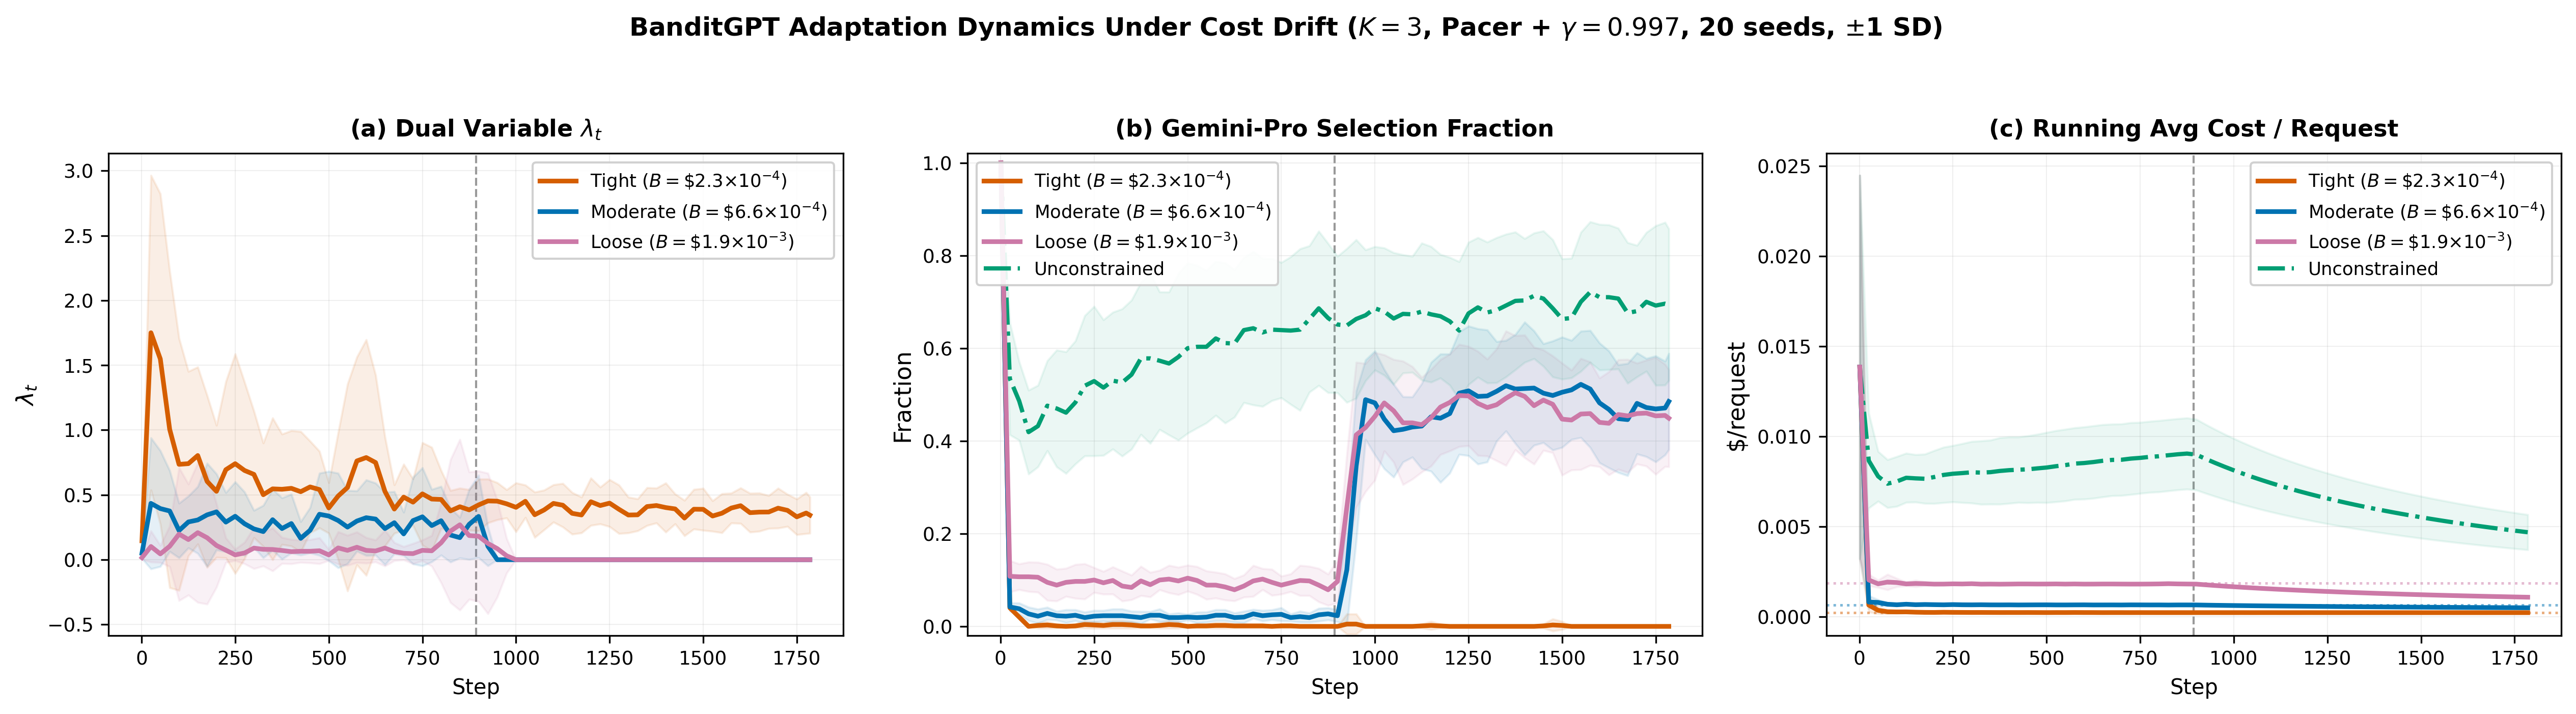
\includegraphics[width=\linewidth]{../experiments_v2/03_budget_plus_drift/results/adaptation_dynamics.pdf}
    \caption{BudgetPacer adaptation under a Gemini price drop at three
    budget levels ($K{=}3$; Pacer + adaptive~$\gamma$; 20~seeds,
    $\pm$1\,SD shading).  The unconstrained BanditGPT baseline (same
    algorithm, same priors, no budget constraint) is shown in green
    dash-dot for comparison.
    %
    \textbf{(a)~Dual variable $\lambda_t$:}
    At moderate budget, $\lambda_t$ drops from ${\sim}0.32$ to
    ${\sim}0.006$ within ${\sim}200$ steps of the price drop
    (step~893).  At loose budget, $\lambda_t$ was already near zero.
    At tight budget, $\lambda_t$ decreases from $0.50$ to $0.37$ but
    remains elevated due to EMA momentum.
    %
    \textbf{(b)~Gemini-Pro selection fraction:}
    At moderate and loose budgets, Gemini selection surges from
    $2$--$10\%$ to ${\sim}78\%$ after the price drop, approaching the
    unconstrained level.  At tight budget, Gemini remains below $2\%$
    due to exploration starvation (Section~\ref{sec:budget_drift}).
    %
    \textbf{(c)~Running average cost per request:}
    All pacer conditions maintain Phase~1 costs within $1\%$ of their
    budget targets (dotted horizontal lines).  Post-drop, costs
    decline below target.  The unconstrained baseline spends
    ${\sim}5$--$39\times$ more.
    }
    \label{fig:exp03_adaptation}
\end{figure*}
